\documentclass[UTF8,a4paper]{ctexart}
\usepackage[utf8]{inputenc}
\usepackage{amsmath}
\usepackage{pdfpages}
\usepackage{graphicx}
\usepackage{wrapfig}
\usepackage{listings}
\title{线控作业1}
\author{张蔚桐\ 2015011493\ 自55}
\begin {document}
\maketitle
\section{}
\section{}
从图\ref{f1ori}中可以预计,系统的传递函数可以表示为$G(s)=\frac{K}{s(T_1s+1)(T_2s+1)},T_1>0,T_2>0$可以根据相频图估计转折频率$\omega_1=18.14\rm{rad/s},\omega_2=1103\rm{rad/s}$可得$T_1=\frac{1}{\omega_1}=0.551\rm{s},T_2=\frac{1}{\omega_2}=0.9066\times 10^{-3}\rm{s}$,同时,考虑辐频在$\omega=1\rm{rad/s}$附近的增益可得$20lg(K)=-9.2;K=0.346$因此系统传递函数可以表示为$$G(s)=\frac{0.346}{s(0.551s+1)(0.9066\times 10^{-3}s+1)}$$,对应的Bode图如图\ref{f1the}所示,可以看出和实际bode图\ref{f1ori}还是基本符合的
\begin{figure}
\centering
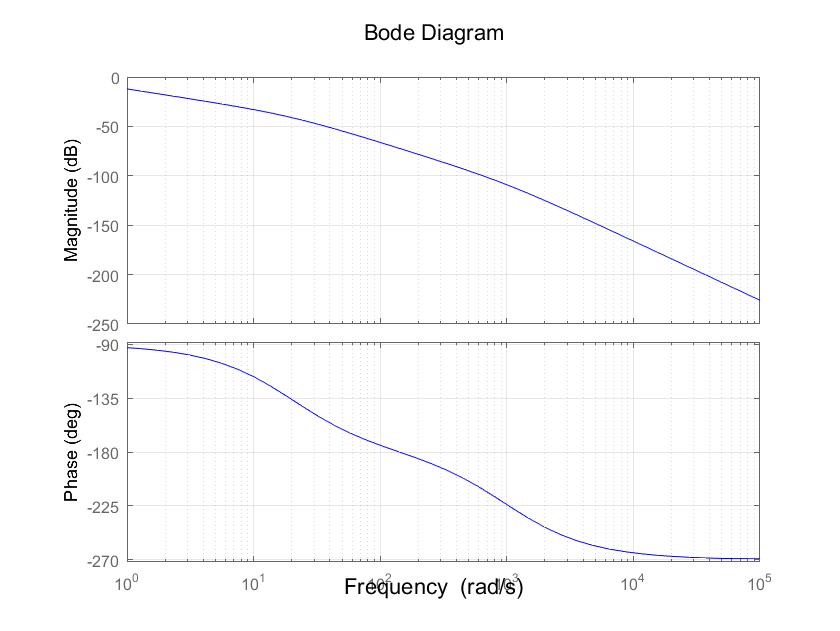
\includegraphics[width=\textwidth]{motorG.jpg}
\caption{原图像}
\label{f1ori}
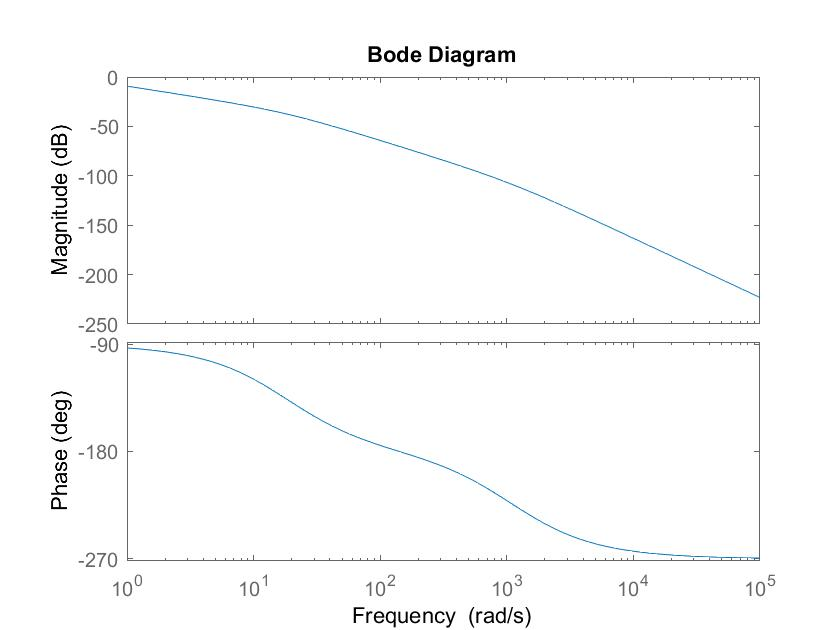
\includegraphics[width=\textwidth]{RmotorG.jpg}
\caption{理论图像}
\label{f1the}
\end{figure}
\section{}
如图\ref{f2ori}显然这是一个惯性环节的图像,可以直接看出$$G(s)=\frac{0.102}{(0.001s+1)}$$MATLAB仿真之后的图像如图\ref{f2the}所示,和原图\ref{f2ori}基本一致
\begin{figure}
\centering
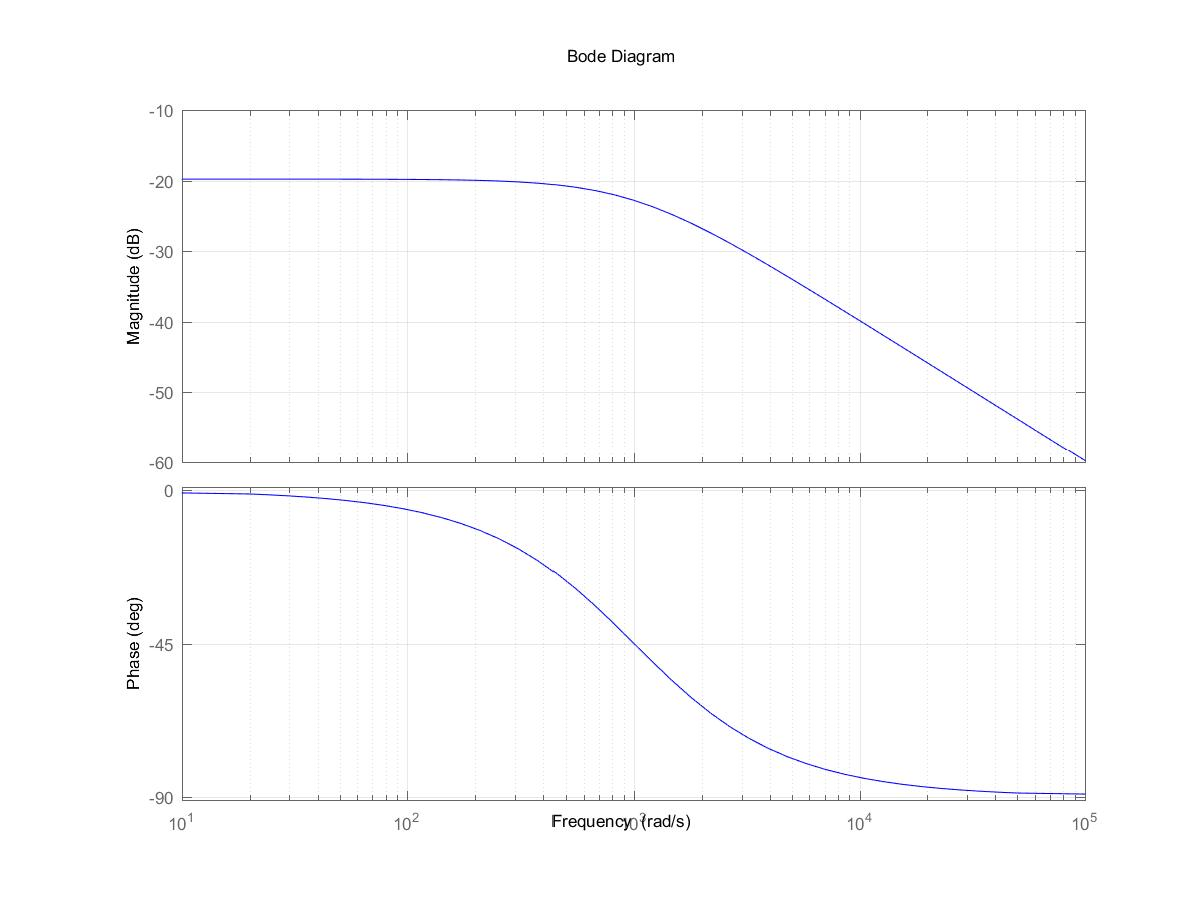
\includegraphics[width=\textwidth]{motorG1.jpg}
\caption{原图像}
\label{f2ori}
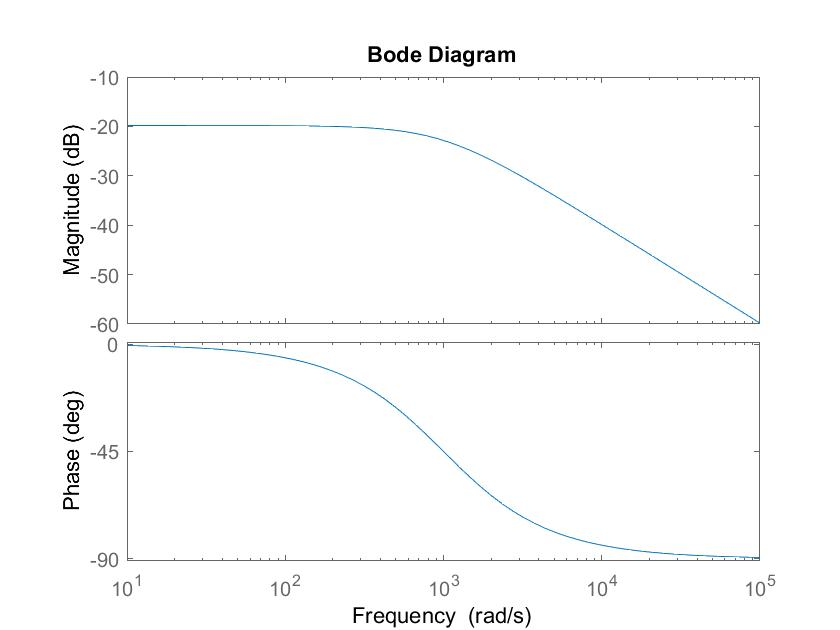
\includegraphics[width=\textwidth]{RmotorG1.jpg}
\caption{理论图像}
\label{f2the}
\end{figure}
\section{}
可以看出系统的传递函数为$G(s)=\frac{K}{s(Ts+1)},T>0$,并由图\ref{f3ori}可以得到$20lg(K)=7.196,K=2.29,T=\frac{1}{20}=0.05$因此$$G(s)=\frac{2.29}{s(0.05s+1)}$$MATLAB作图如图\ref{f3the}所示,和实际情况相差不多
\begin{figure}
\centering
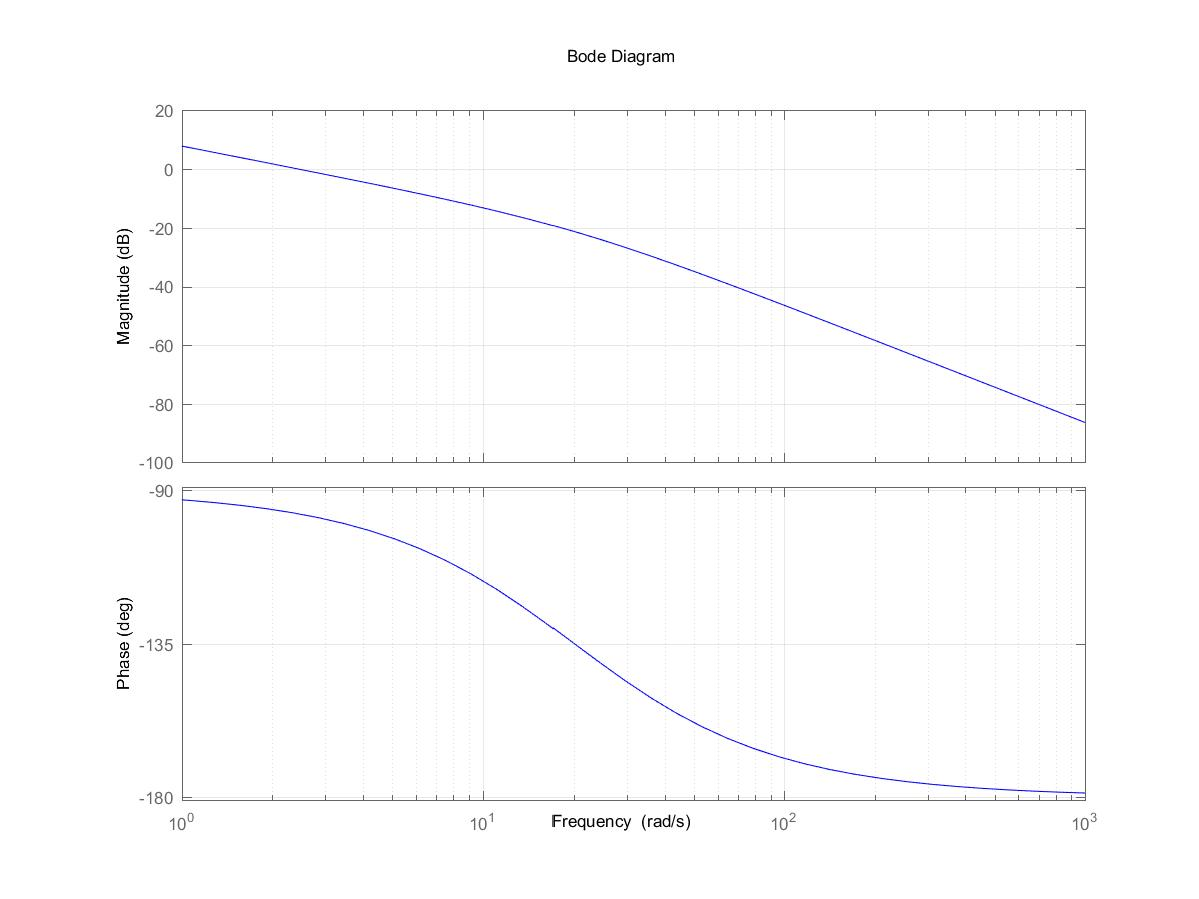
\includegraphics[width=\textwidth]{motorG2.jpg}
\caption{原图像}
\label{f3ori}
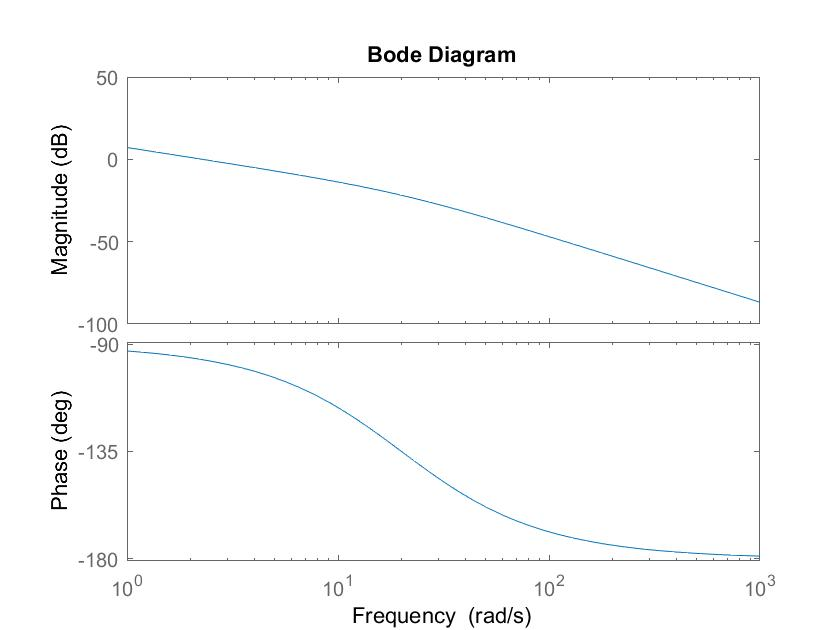
\includegraphics[width=\textwidth]{RmotorG2.jpg}
\caption{理论图像}
\label{f3the}
\end{figure}
\section{}
\section{}
\section{}
\section{}
\section{}
\section{}
\section{}
\section{}
\section{}
\section{}
\section{}
\section{}
\section{}
\end{document}